\documentclass[10pt, reqno]{amsart}
\usepackage[margin = 0.5 in]{geometry}
\usepackage{multicol}
\usepackage{float}
\usepackage{fancyhdr}
\usepackage{graphicx}
\usepackage{hyperref}
\usepackage{fancyvrb}
\usepackage{physics}

\setlength{\abovecaptionskip}{5pt plus 3pt minus 3pt}

\hypersetup{colorlinks=true,allcolors=blue}
\pagestyle{fancy} \fancyhead{} \fancyfoot[C]{\normalsize\thepage}
\renewcommand{\headrulewidth}{0pt}
\begin{document}
\title{ME 5311 \quad Assignment 3 \quad Jacob Ivanov}

\maketitle
\begin{multicols}{2}
    \section{Finite Difference}
    In order to find a finite difference approximation of the following form, we can use a Taylor Table. 
    \begin{equation}
        \left( \pdv{u}{x} \right)_i = \frac{1}{\Delta x} \Big( a u_{i - \frac{3}{2}} + b u_{i - \frac{1}{2}} + c u_{i + \frac{1}{2}} \Big)
    \end{equation}
    
    \begin{center}
        \begin{tabular}{ c | c c c c}
          & $u_i$ & $\Delta x \left( \pdv{u}{x} \right)_i$ & $\Delta x^2 \left( \pdv[2]{u}{x} \right)_i$ & $\Delta x^3 \left( \pdv[3]{u}{x} \right)_i$ \\ 
          \hline\\
          $\Delta x \left( \pdv{u}{x} \right)_i$ & 0 & 1 & 0 & 0 \\
          \\
          $-a u_{i - \frac{3}{2}}$ & $-a$ & $+\frac{3}{2} a$ & $-\frac{9}{8} a$ & $+\frac{27}{48} a$ \\
          \\
          $-b u_{i - \frac{1}{2}}$ & $-b$ & $ + \frac{1}{2} b$ & $ -\frac{1}{8} b$ & $ +\frac{1}{48} b$ \\
          \\
          $-c u_{i + \frac{1}{2}}$ & $-c$ & $-\frac{1}{2} c$ & $-\frac{1}{8} c$ & $- \frac{1}{48} c$ \\
        \end{tabular}
    \end{center}
    By summing the first three columns, we can obtain the following linear system and solution:
    \begin{equation}
        \begin{bmatrix}
            1 & 1 & 1\\
            3/2 & 1/2 & -1/2\\
            9/8 & 1/8 & 1/8
        \end{bmatrix} \begin{bmatrix}
            a \\ b \\ c
        \end{bmatrix} = \begin{bmatrix}
            0 \\ -1 \\ 0
        \end{bmatrix} \to \begin{bmatrix}
            a \\ b \\ c
        \end{bmatrix} = \begin{bmatrix}
            0 \\ -1 \\ +1
        \end{bmatrix}
    \end{equation}
    \begin{equation}
        \left( \pdv{u}{x} \right)_i = \frac{1}{\Delta x} \Big( -u_{i - \frac{1}{2}} + u_{i + \frac{1}{2}} \Big)
    \end{equation}
    An error bound for this approximation can be found by summing the last column, multiplying by the heading term, and dividing by $\Delta x$:
    \begin{equation}
        E = \frac{\Delta x^3 \left( \pdv[3]{u}{x} \right)_i}{\Delta x} \Big( \frac{27}{48}(0) - \frac{1}{48}(2) \Big) = - \frac{\Delta x^2}{24} \left( \pdv[3]{u}{x} \right)_i
    \end{equation}
    Equation (3) was also verified by differentiating the Lagrange Interpolating Polynomial of these three point/position values, which was simplified using Mathematica (note that there was a change of variables from $u \to f$):
    \begin{figure}[H]
        \centering
        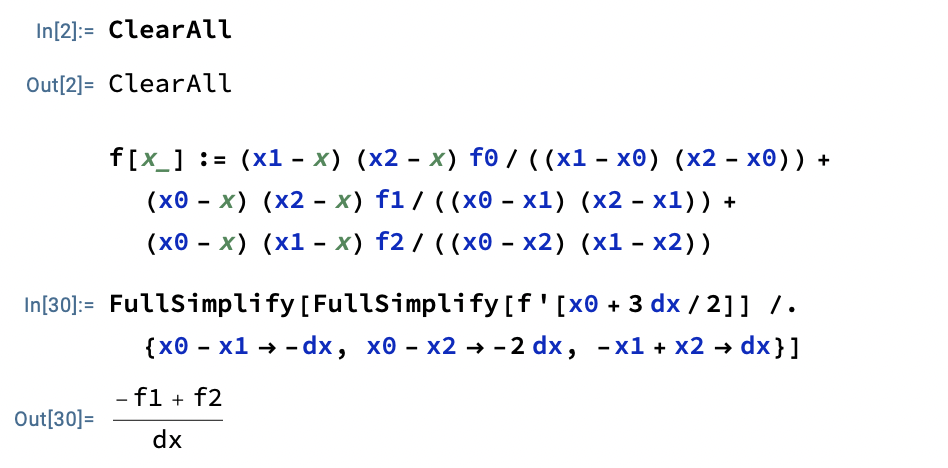
\includegraphics[width=1\linewidth]{Derivation of FD Approximation.png}
    \end{figure}
    It can be seen that these two are equivalent. A Lagrange Interpolating Polynomial with 3 points is of order 2, which agrees with the error estimate.

    \section{Numerical Error}
    The following integral was numerically evaluated and a convergence test was completed against the analytical result:
    \begin{equation}
        A = \int_0^1 x^{\frac{3}{2}} \,\dd x = \frac{2}{5}
    \end{equation}
    \begin{figure}[H]
        \centering
        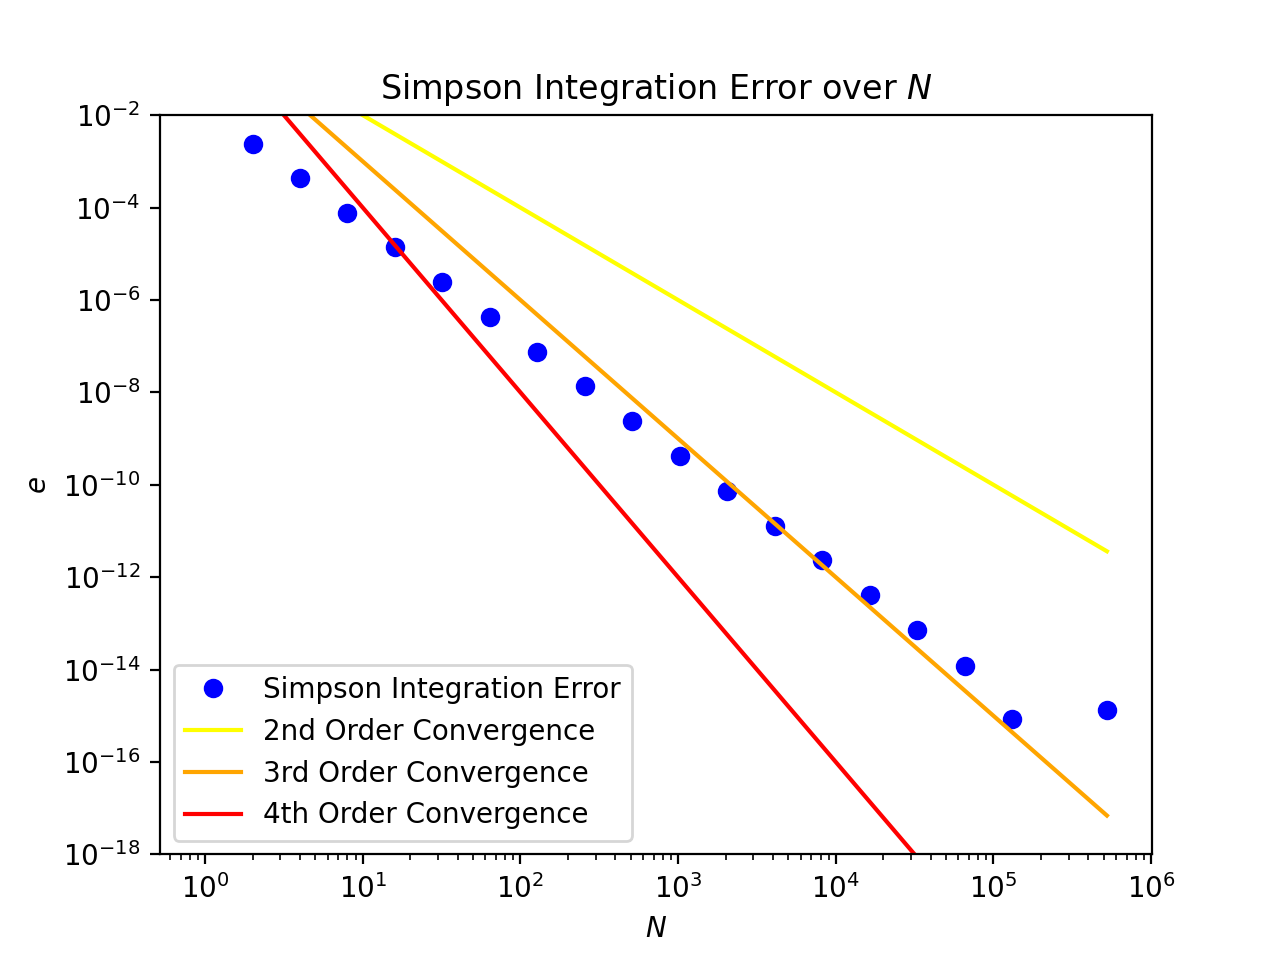
\includegraphics[width=1\linewidth]{Simpson Integration Error over N.png}
    \end{figure}
    It can be seen that this integral numerically converges at roughly order 2.5, which is in inconsistent with the convergence rate of Simpson's Rule, which should be of order 4. This is due to the fact that the 2nd, 3rd, and 4th derivatives are unbounded as $x \to 0^+$.

    \section{Runge-Kutta Method}
    \begin{figure}[H]
        \centering
        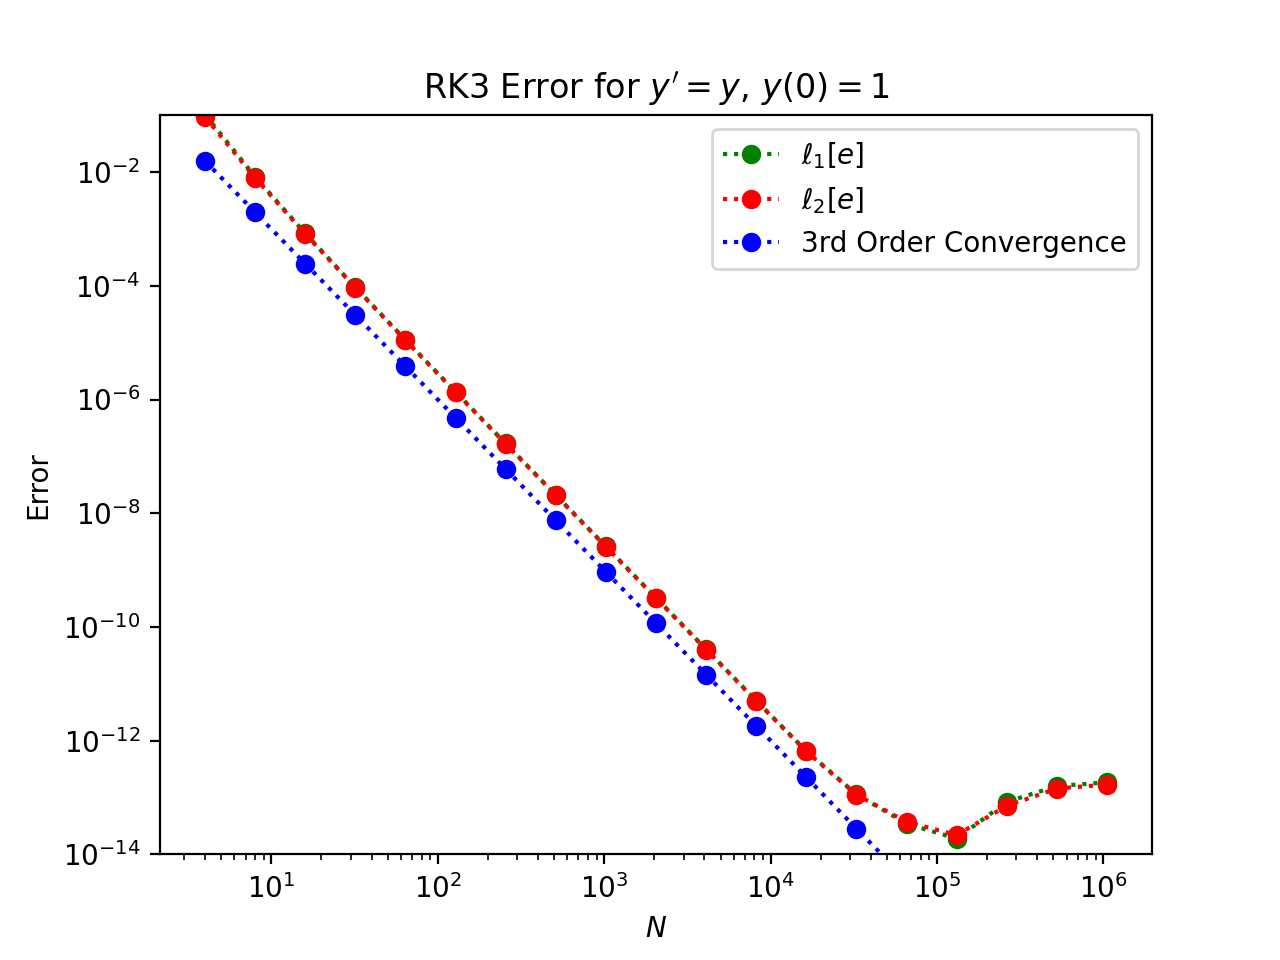
\includegraphics[width=1\linewidth]{RK3 Error Convergence (exp).png}
    \end{figure}
    Integrating the ODE $y = y'$ yields the known analytical solution $y = e^t$, and numerically integrating this ODE with a 3rd Order Runge-Kutta method shows the expected 3rd Order Convergence rate. It should be noted that the $\ell_1$ and $\ell_2$ norms are almost identical values, such that the two plot series lie almost directly on top of one another. They have the same convergence rate as well.

    Integrating the Lorenz System, we obtain the following:
    \begin{figure}[H]
        \centering
        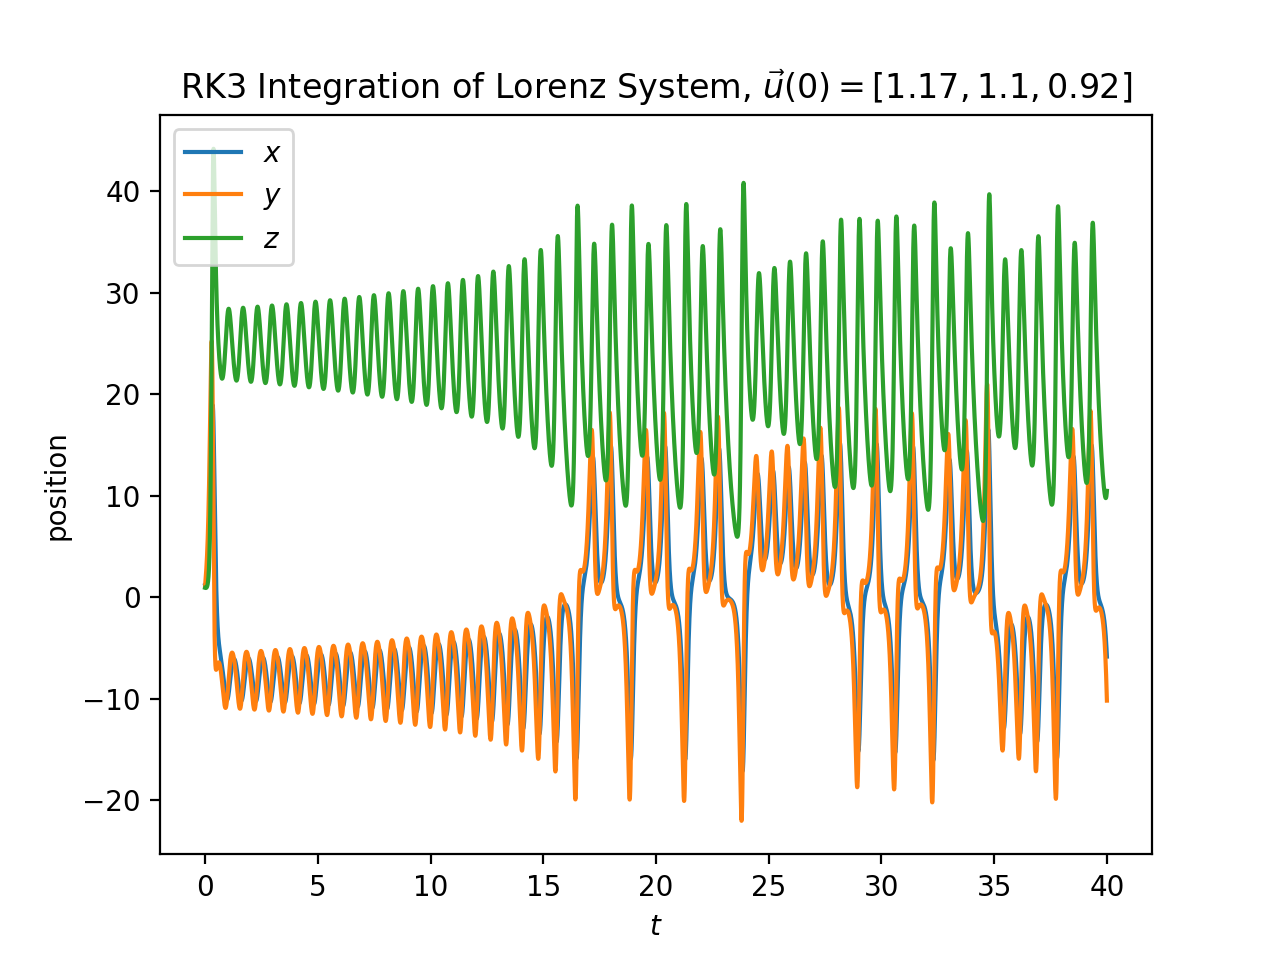
\includegraphics[width=1\linewidth]{RK3 Integration of Lorenz System.png}
    \end{figure}
    Perturbing the initial position by 1\% results in the positions to be relatively similar for some time, prior to complete divergence, as shown below:
    \begin{figure}[H]
        \centering
        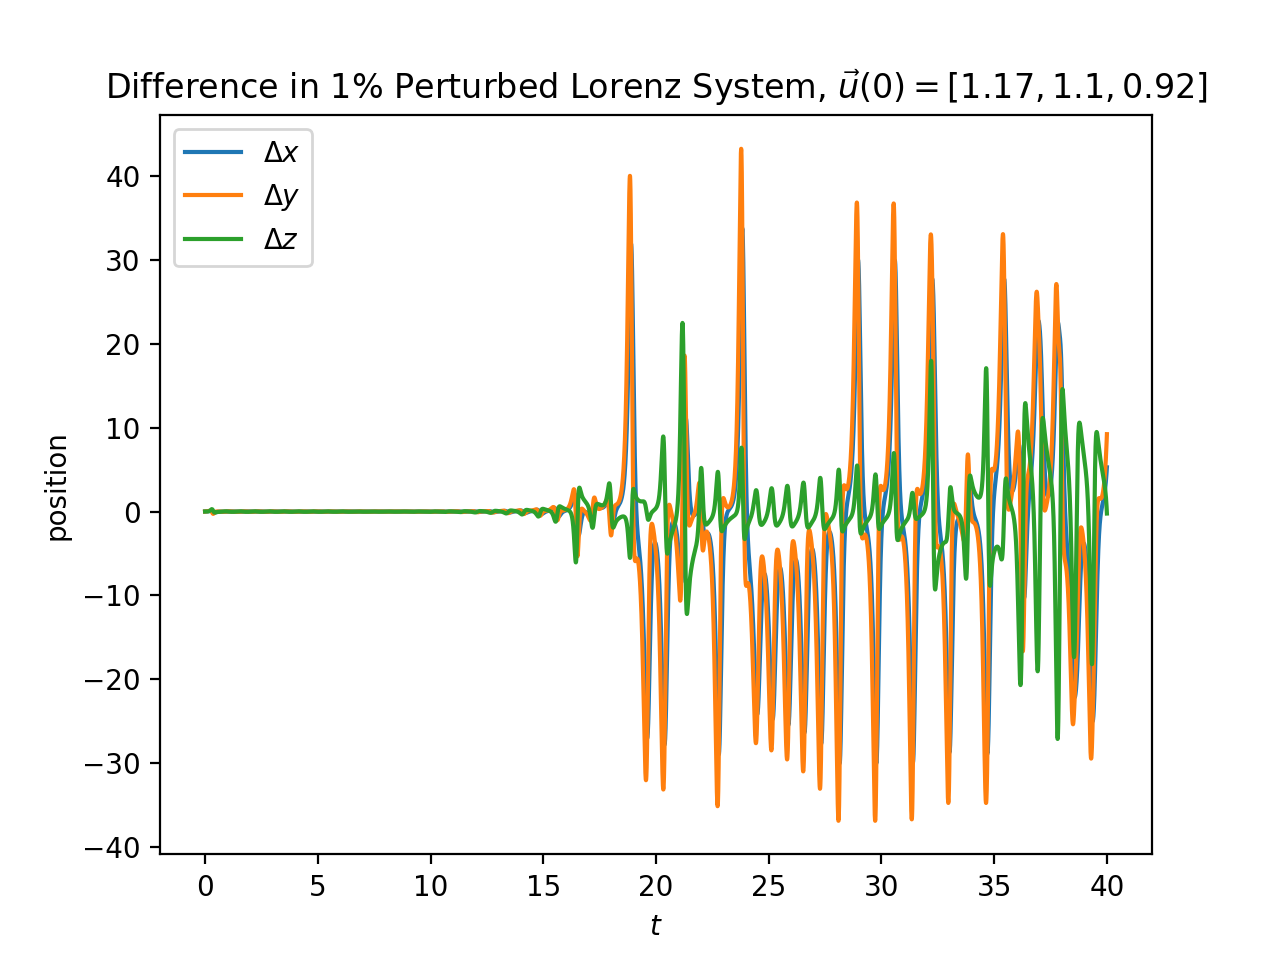
\includegraphics[width=1\linewidth]{Difference in 1 Perturbed Lorenz System.png}
    \end{figure}
\end{multicols}
\end{document}